\documentclass[a4paper,12pt]{article}
 \usepackage[utf8]{inputenc}
 \usepackage[left=2cm,top=1cm,right=2cm,bottom=1.5cm,nohead]{geometry}
%\usepackage{wrapfig} % Обтекание рисунков текстом
%\usepackage{floatflt}% Обтекание таблиц текстом
 \usepackage{amsmath} % Математические окружения AMS
 \usepackage{amsfonts} % Шрифты AMS
 \usepackage{amssymb} % Символы AMS
 \usepackage{listings}% to add computer code
 \usepackage{color}
 \definecolor{mygreen}{RGB}{28,172,0} % color values Red, Green, Blue
\definecolor{mylilas}{RGB}{170,55,241}
    \usepackage{graphicx} % Вставить pdf- или png-файлы
  \usepackage{euscript} % Красивый шрифт
%\usepackage{extsizes} % Возможность сделать 14-й шрифт
 \linespread{1.5} % Интерлиньяж
% \usepackage[usenames,dvipsnames,svgnames,table,rgb]{xcolor}% чтоб были гиперссылки и чтоб были цвета

\usepackage{hyperref} % Гиперссылки

%\hypersetup{
% colorlinks = true,
 %linkcolor = MidnightBlue, % ссылки на всякие разделы (их цвет)
 %urlcolor = [rgb]{0,0,1}, % чтоб задавать цыета пиксела - red green blue. не рекомендуется, если потом печатать.
 %citecolor = black
%}
%\usepackage{pdflscape}
%\oddsidemargin=10mm
%\topmargin=-15mm
\usepackage{multicol}
%\hoffset=5mm % см при печати
%\voffset=4.2mm
%\textheight = 720pt
%\textwidth=442pt

\begin{document}
\maketitle \hrulefill
\lstset{language=Matlab,%
    %basicstyle=\color{red},
    breaklines=true,%
    morekeywords={matlab2tikz},
    keywordstyle=\color{blue},%
    morekeywords=[2]{1}, keywordstyle=[2]{\color{black}},
    identifierstyle=\color{black},%
    stringstyle=\color{mylilas},
    commentstyle=\color{mygreen},%
    showstringspaces=false,%without this there will be a symbol in the places where there is a space
    numbers=left,%
    numberstyle={\tiny \color{black}},% size of the numbers
    numbersep=9pt, % this defines how far the numbers are from the text
    emph=[1]{for,end,break},emphstyle=[1]\color{red}, %some words to emphasise
    %emph=[2]{word1,word2}, emphstyle=[2]{style},
}

\begin{center}

\textbf {\Large{Empirircal Methods HA 6}}\\
Konstantin Guryev\\
Pennsylvania State University\\
2019
\end{center}

\textbf{Problem \textnumero \,1 }

\vspace{\baselineskip}
The Bellman equation is of the form:
$$V(p,x) = \max\limits_{x'\in [0,x]}\{p(x-x')-\frac{1}{5}(x-x')^{\frac{3}{2}} + \delta \mathds{E}_{p'|p}V(p',x')\}$$,
%\vspace{\baselineskip}
$$p' = \frac{1}{2} + \frac{1}{2}p + \epsilon, \delta = 0.95,  x \in [0,100], \epsilon \sim N(0, 0.01)$$

A pair $(p,x)$ is a state variable, where $p$ is a price at a given time period and $x$ is a stock of lumber in the firm. $x'$ is a stock of lumber at the next period, which is our policy variable. Price follows an AR(1) process.

\textbf{Problem \textnumero \,2 }

%\vspace{\baselineskip}
See the code. 
%\vspace{\baselineskip}
\newpage
\textbf{Problem \textnumero \,3 }


\begin{figure}[h]
\centering
%\begin{center}
\includegraphics[width=16cm,height=8cm,keepaspectratio]{Pr3_figure.eps}
%\caption{Движущийся жесткий штамп}
%\caption{pic1}
%\end{center}
\end{figure}



\textbf{Problem \textnumero \,4 }

\vspace{\baselineskip}
\begin{figure}[h]
\centering
\includegraphics[width=16cm,height=8cm,keepaspectratio]{Pr4_figure.eps}
%\caption{pic1}
\end{figure}
\vspace{\baselineskip}
\newpage

\textbf{Problem \textnumero \,5 }

\vspace{\baselineskip}
One may see that the confidence interval tends to expand over time. This result is natural since the further we are in the future the more uncertainty we face.

\begin{figure}[h]
\centering
\includegraphics[width=16cm,height=8cm,keepaspectratio]{Pr5_figure.eps}
%\caption{pic1}
\end{figure}
\vspace{\baselineskip}
\newpage
\textbf{Problem \textnumero \,6}

One may notice that on this grid the distance between the graphs of the value functions for the different prices is becoming larger when the price increases in comparison with the finer grid. Everything else seems to be pretty the same, therefore 5 points is also quite good a grid.


\begin{figure}[h]
\centering
\includegraphics[width=16cm,height=8cm,keepaspectratio]{Pr6_figure1.eps}
%\caption{pic1}
\end{figure}

\begin{figure}[h]
\centering
\includegraphics[width=16cm,height=8cm,keepaspectratio]{Pr6_figure2.eps}
%\caption{pic1}
\end{figure}








\newpage
\section*{Matlab Code} \lstinputlisting{tauchen.m}
\newpage
\section*{Matlab Code} \lstinputlisting{u.m}
\newpage
\section*{Matlab Code} \lstinputlisting{HA_6_Guryev.m}


\end{document}